\newpage
\section*{Appendix}

\section{Additional Related Dataset Work}\label{app:related}
Existing datasets~\cite{atzeni2017fine,xu2018stock,rodrigues2019combining,farimani2021leveraging,sinha2022sentfin,dong2024fnspid,cao2023tempo} primarily focus on stock analysis tasks in the finance domain. Other multi-modal datasets for traffic demand prediction~\cite{rodrigues2019combining}, news impact prediction~\cite{jia2024gpt4mts} and electrocardiogram classification~\cite{li2024frozen} are proposed recently. However, these datasets still do not address the aforementioned gaps. Especially constructing datasets for diverse domains, such as agriculture and security, is more challenging but holds substantial real-world impact.


Besides, some datasets focus on combining images with numerical sequences, where the images are typically
sourced from spatial domains, such as satellite imagery. These works ~\cite{gerard2023wildfirespreadts,liu2012spatial} are centered on spatiotemporal data
analysis, whereas our work focuses on time series analysis.

Additional multi-modal datasets~\cite{jia2024gpt4mts} for news impact prediction and electrocardiogram classification~\cite{li2024frozen} are proposed recently. However, these datasets still do not address the aforementioned gaps. Especially constructing multimodal datasets for other domains, such as agriculture and security, is more challenging but holds substantial real-world impact.
\section{Limitations}\label{app:limitaion}
Our work provides a comprehensive, high-quality multimodal time series dataset, but it still has limitations in terms of dataset diversity, as all the text data comes from English. We plan to extend \model to multilingual versions to better address diversity and leverage data from multiple languages~\cite{jin2024better}.  In addition, utilizing \model to support other multimodal time series analysis tasks, such as multivariate time series forecasting and time series classification, requires additional dataset curation work.  Moreover, considering multimodal time series datasets with images and audio is a worthwhile direction for future work. In this work, we chose to include text for the following reasons: (1) Text and numerical series commonly coexist across multiple domains. (2) With the rise of LLMs, an increasing number of time-series methods are incorporating text based on large language models. Collecting data that further align images~\cite{gerard2023wildfirespreadts} ,audio~\cite{kashino1999time} or graph~\cite{liu2021signed} with text and numeric is meaningful but beyond the scope of this work. Lastly, this work focuses on time series forecasting and does not cover interacting dynamical systems or equation discovery~\cite{liuamortized}, where language could provide insights into the qualitative behavior of the system.

Our multimodal time series forecasting library is built upon a simple integration framework that only uses a projection layer for fine-tuning LLMs. How to fine-tune LLMs more efficiently and effectively for time series analysis remains an interesting topic. Moreover, addressing the issue of distributional shift~\cite{zhang2022towards,zhao2023performative,liu2024time} in the text should also be considered in future work to build robust models. In summary, our approach to achieve multimodal time series forecasting based on \model dataset is a first-cut reasonable approach rather than the optimal solution. There could be better ways to utilize it, such as Retrieval-Augmented Generation~\cite{gao2023retrieval}.









Despite these limitations, we hope that the datasets and library we have constructed will facilitate broader research and applications in multimodal time series analysis, such as benchmark~\cite{jin2024mm} and agent~\cite{jin2024agentreview}.
\section{Considerations for Domain Selection}\label{app:domain}
Our domain selection is based on the following three considerations:
\begin{itemize}
    \item Most of our selected domains are also widely used in existing time-series works~\cite{liutimer,ansari2024chronos,dasdecoder,woounified}
 but lack textual and numerical alignment. We chose these domains to facilitate comparison by researchers, and all these domains have significant real-world importance.
    \item The remaining three domains, including social good, agriculture, and security, are often overlooked by researchers. We included these domains to contribute to a more comprehensive dataset.
    \item Additionally, we also considered underrepresented groups, as reflected in the Health (Africa) dataset, compared with the Health (U.S.).
\end{itemize}
These domains exhibit differences in numerical data, textual data, and performances. To the best of our knowledge, our Time-MMD is the most domain-inclusive multimodal time-series dataset. 

\section{Details of Data Sources and Variables by Domain}\label{app:data source}
\subsection{Agricultural Domain Dataset Sources}


\subsubsection{Numeric Data}
The sequence raw data is sourced from the \textit{retail broiler composite}, provided by the United States Department of Agriculture (USDA) Economic Research Service (ERS). The raw data can be accessed at the USDA ERS website\footnote{\url{https://www.ers.usda.gov/data-products/meat-price-spreads/documentation/}}.

\subsubsection{Text Data}
\paragraph{Report: Source 1}
\begin{itemize}
    \item \textbf{Frequency:} Weekly
    \item \textbf{Name:} USDA Broiler Market News Report.
    
    \item \textbf{URL:} \url{https://usda.library.cornell.edu/concern/publications/5999n3392?locale=en&page=30#release-items}.
    
    \item \textbf{Description:} This report provides a summary of the national broiler market, with data consolidated from a number of linked reports. The release contains price information for broiler parts by U.S. region as well as in Mexico City, slaughter estimates, availability, and national fowl market and miscellaneous poultry information.
\end{itemize}

\paragraph{Report: Source 2}
\begin{itemize}
    \item \textbf{Frequency:} Daily
    \item \textbf{Name:} Daily National Broiler Market at a Glance.
    
    \item \textbf{URL:} \url{https://usda.library.cornell.edu/concern/publications/vx021f146?locale=en&page=142#release-items}.
    
    \item \textbf{Description:} This report summarizes the daily trends in the national broiler market, with commentary on price, demand and supply, market activity, and trade.
\end{itemize}
\paragraph{Search}
\begin{itemize}
    \item \textbf{Frequency:} 10 results per week.
    \item \textbf{Keywords:} United States Broiler Market; Chicken prices 
\end{itemize}


 \subsection{Climate  Domain Dataset Sources}
The data is collected by the NOAA National Centers for Environmental Information and spans from 1895 to the present. It offers a comprehensive historical dataset for analyzing long-term climate trends and their implications for energy and environmental policies. The raw data can be accessed at the NOAA.

\subsubsection{Numeric Data}
\paragraph{Source}:\url{https://www.drought.gov/historical-information?dataset=0&selectedDateUSDM=20240514}

\subsubsection{Text Data}
\paragraph{Report: Source 1}
\begin{itemize}
    \item \textbf{Frequency:} Month
    \item \textbf{Name:} Drought Report of NOAA National Centers for Environmental Information\footnote{\url{https://www.ncei.noaa.gov/access/monitoring/monthly-report/drought/200602}}.
    \item \textbf{Description:} Drought Highlights;National Overview;Regional Overview

\end{itemize}
\paragraph{Report: Source 2}
\begin{itemize}
    \item \textbf{Frequency:} Month
    \item \textbf{Name:} National Climate Report of NOAA National Centers for Environmental Information\footnote{\url{https://www.ncei.noaa.gov/access/monitoring/monthly-report/national/200602}}.
    \item \textbf{Description:} National Overview;Monthly and Seasonal Highlights;
\end{itemize}
\paragraph{Search}
\begin{itemize}
    \item \textbf{Frequency:} 10 results per week.
    \item \textbf{Keywords:} Drought and extreme weather; Precipitation
\end{itemize}
\subsection{Economy  Domain Dataset Sources}


\subsubsection{Numeric Data}
\paragraph{Source}:\url{https://www.census.gov/foreign-trade/balance/c0015.html}.

\subsubsection{Text Data}
\paragraph{Report: Source 1}
\begin{itemize}
    \item \textbf{Frequency:} Monthly
    \item \textbf{Name:} U.S. International Trade in Goods and Services \footnote{\url{https://www.census.gov/foreign-trade/Press-Release/ft900_index.html}}.
\end{itemize}
\paragraph{Report: Source 2}
\begin{itemize}
    \item \textbf{Frequency:} Monthly
    \item \textbf{Name:} Advance Economic Indicators Report\footnote{\url{https://www.census.gov/econ/indicators/current/index.html}}.
\end{itemize}
\paragraph{Search}
\begin{itemize}
    \item \textbf{Frequency:} 10 results per week.
    \item \textbf{Keywords:} International Trade Balance
\end{itemize}
\subsection{Energy Domain Dataset Sources}

This subsection outlines the sources and characteristics of the sequence and raw textual data that form the energy component of the series-text dataset. This domain specifically focuses on gasoline prices, which are crucial for analyzing economic stability, consumer spending patterns, and the overall energy market dynamics.

\subsubsection{Numeric Data}
The sequence raw data comprises weekly statistics of U.S. gasoline prices, measured in dollars per gallon. Monitoring these prices provides insights into energy market fluctuations and helps predict changes in economic conditions and policy adjustments.

\paragraph{Source and Accessibility}
This data is collected by the U.S. Energy Information Administration (EIA) and spans from April 5, 1993, to the present, offering a comprehensive historical view of fuel economics. The raw data can be accessed at the EIA website\footnote{\url{https://www.eia.gov/petroleum/gasdiesel/}}.

\subsubsection{Text Data}
We collect raw text from various EIA publications and reports, as they provide contextual information and expert analysis related to the Numeric Data. 


\paragraph{Report Source 1: Annual Energy Outlook}
\begin{itemize}
    \item \textbf{Frequency:} Annually
    \item \textbf{Source:} U.S. Energy Information Administration\footnote{\url{https://www.eia.gov/outlooks/aeo/archive.php}}.
    \item \textbf{Type:} Annual Energy Outlook reports
    \item \textbf{Coverage:} From 1979 to present
\end{itemize}

\paragraph{Report Source 2: Weekly Petroleum Status Report}
\begin{itemize}
    \item \textbf{Frequency:} Weekly
    \item \textbf{Source:} U.S. Energy Information Administration\footnote{\url{https://www.eia.gov/petroleum/supply/weekly/archive/}}.
    \item \textbf{Type:} Weekly Petroleum Status Reports
    \item \textbf{Coverage:} From 2011 to present
\end{itemize}
\paragraph{Search}
\begin{itemize}
    \item \textbf{Frequency:} 10 results per week.
    \item \textbf{Keywords:} Gasoline prices
\end{itemize}



\subsection{Social Good Domain Dataset Sources}

This subsection describes the sources and characteristics of the sequence and raw textual data that comprise the social good component of the series-text dataset. This domain focuses on unemployment statistics in the United States, segmented by various racial groups, reflecting the societal impact of economic disparities.

\subsubsection{Numeric Data}
The sequence raw data consists of monthly unemployment statistics for the United States, disaggregated by race. These statistics include data for the following racial groups: White, Black or African American, Asian, American Indian or Alaska Native, and Native Hawaiian or Other Pacific Islander.

This data is sourced from the United States Bureau of Labor Statistics (BLS) and spans from 1954 to the present, providing a long-term view of employment trends across different racial demographics. The raw data can be accessed at the BLS website\footnote{\url{https://data.bls.gov/home.htm}}.

\subsubsection{Text Data}
The raw textual data is sourced from official reports which provide a comprehensive analysis of employment conditions, enriched with context that is crucial for understanding the nuances of unemployment across different racial groups.

\paragraph{Report Source 1}

\begin{itemize}
    \item \textbf{Frequency:} Monthly
    \item \textbf{Source:} U.S. Department of Labor, BLS\footnote{\url{https://www.bls.gov/bls/news-release/empsit.htm}}.
    \item \textbf{Type:} Official report on monthly employment situations
    \item \textbf{Coverage:} From 1994 to present
    \item \textbf{Quantity:} TBD
    \item \textbf{Relevance:} Directly relevant (Siamese)
\end{itemize}

\paragraph{Report Source 2}
\begin{itemize}
    \item \textbf{Frequency:} Annually
    \item \textbf{Source:} U.S. Department of Labor, BLS\footnote{\url{https://www.bls.gov/opub/reports/race-and-ethnicity/2015/home.htm}}.
    \item \textbf{Type:} Official report on annual labor force characteristics by race and ethnicity
    \item \textbf{Coverage:} From 2015 to present
    \item \textbf{Quantity:} TBD
    \item \textbf{Relevance:} Directly relevant
\end{itemize}
\paragraph{Search}
\begin{itemize}
    \item \textbf{Frequency:} 10 results per week.
    \item \textbf{Keywords:} Unemployment rate; Employment situation
\end{itemize}


\subsection{Public Health (United States) Domain Dataset Sources}

This subsection outlines the sources and characteristics of the sequence and raw textual data that form the public health component of the series-text dataset. This domain specifically focuses on Influenza-Like Illness (ILI) statistics, which are crucial for monitoring seasonal and pandemic influenza outbreaks, guiding public health interventions, and planning healthcare resources effectively.

\subsubsection{Numeric Data}
The sequence raw data includes weekly statistics of ILI cases in the United States, sourced from the Centers for Disease Control and Prevention (CDC). ILI, representing a category of health conditions characterized by symptoms similar to those of influenza, serves as an important public health indicator for tracking influenza activity.

\paragraph{Source and Accessibility}
The data is collected and made available by the CDC's ILINet system, which has been tracking ILI cases since 1954. This extensive dataset allows for robust historical trend analysis and modeling of influenza patterns. The raw influenza patients data can be accessed at the CDC website\footnote{\url{https://gis.cdc.gov/grasp/fluview/fluportaldashboard.html}}.

\subsubsection{Text Data}
Raw textual data in the public health domain includes official reports and related news, providing insights into the context and implications of the ILI statistics.

\paragraph{Report Source 1: Weekly U.S. Influenza Surveillance Report}
\begin{itemize}
    \item \textbf{Frequency:} Weekly
    \item \textbf{Source:} CDC\footnote{\url{https://www.cdc.gov/flu/weekly/pastreports.htm}}.
    \item \textbf{Type:} Official Weekly U.S. Influenza Surveillance Report
    \item \textbf{Coverage:} From 1999 to present
\end{itemize}

\paragraph{Report Source 2: Annual Flu Season Key Studies and News Reports}
\begin{itemize}
    \item \textbf{Frequency:} Annually
    \item \textbf{Source:} CDC\footnote{\url{https://www.cdc.gov/flu/spotlights/index.htm}}.
    \item \textbf{Type:} Key studies and news reports from the flu season
    \item \textbf{Coverage:} From 2019 to present
\end{itemize}
\paragraph{Search}
\begin{itemize}
    \item \textbf{Frequency:} 10 results per week.
    \item \textbf{Keywords:} influenza; epidemic
\end{itemize}

\subsection{Public Health (Africa)  Domain Dataset Sources}


\subsubsection{Numeric Data}
\paragraph{Source:} World Health Organization \footnote{\url{https://app.powerbi.com/view?r=eyJrIjoiNjViM2Y4NjktMjJmMC00Y2NjLWFmOWQtODQ0NjZkNWM1YzNmIiwidCI6ImY2MTBjMGI3LWJkMjQtNGIzOS04MTBiLTNkYzI4MGFmYjU5MCIsImMiOjh9}}.

\subsubsection{Text Data}
\paragraph{Report: Source 1}
\begin{itemize}
    \item \textbf{Frequency:} Weekly
    \item \textbf{Name:} Influenza Virological Surveillance in the WHO African Region\footnote{\href{https://www.afro.who.int/publications/influenza-virological-surveillance-who-african-region-epidemiological-week-39-2017}{https://www.afro.who.int/publications/influenza-virological-surveillance-who-african-region-epidemiological-week-39-2017}}.
\end{itemize}
\paragraph{Report: Source 2}
\begin{itemize}
    \item \textbf{Frequency:} Daily
    \item \textbf{Name:} Press of  Africa Centres for Diseases Control\footnote{\url{https://africacdc.org/news-item/africa-centres-for-diseases-control-and-prevention-launches-new-networks-to-fight-health-threats-in-africa/}}.
    \item \textbf{Description:} 
\end{itemize}
\paragraph{Search}
\begin{itemize}
    \item \textbf{Frequency:} 10 results per week.
    \item \textbf{Keywords:} influenza; epidemic
\end{itemize}



\subsection{Environment  Domain Dataset Sources}


\subsubsection{Numeric Data}
\paragraph{Source}:\url{https://www.epa.gov/outdoor-air-quality-data}.

\subsubsection{Text Data}
\paragraph{Report: Source 1}
\begin{itemize}
    \item \textbf{Frequency:} Daily
    \item \textbf{Name:} Press about Air Quality of Department of Environmental Conservation of New York\footnote{\href{https://dec.ny.gov/news/press-releases/2021/5/dec-directs-pvs-chemical-solutions-inc-to-temporarily-cease-operations\%23:~:text=The\%20New\%20York\%20State\%20Department\%20of\%20Environmental\%20Conservation,Medaille\%20College\%20Sports\%20Complex\%20at\%20Buffalo\%20Color\%20Park.}{https://dec.ny.gov/news/press-releases/2021/5/dec-directs-pvs-chemical-solutions-inc-to-temporarily-cease-operations}}.
\end{itemize}
\paragraph{Report: Source 2}
\begin{itemize}
    \item \textbf{Frequency:} Daily
    \item \textbf{Name:} Article about air quality from New York National Broadcasting Company\footnote{\url{https://www.nbcnewyork.com/tag/air-quality/}}.
\end{itemize}
\paragraph{Search}
\begin{itemize}
    \item \textbf{Frequency:} 10 results per week.
    \item \textbf{Keywords:} New York air quality; New York air pollution
\end{itemize}


\subsection{ Traffic Domain Dataset Sources}


\subsubsection{Numeric Data}
\paragraph{Source}:\url{https://www.fhwa.dot.gov/policyinformation/travel_monitoring/tvtfaq.cfm}.

\subsubsection{Text Data}
\paragraph{Report: Source 1}
\begin{itemize}
    \item \textbf{Frequency:} Weekly
    \item \textbf{Name:} Weekly Traffic Volume Report\footnote{\href{https://datahub.transportation.gov/stories/s/Weekly-Traffic-Volume-Report/3g63-ik4u/}{https://datahub.transportation.gov/stories/s/Weekly-Traffic-Volume-Report/3g63-ik4u/}}.
    \item The Traffic Volume report estimates the vehicle miles traveled (VMT) for interstate highways and how the total travel measured by VMT compares with travel that occurred in the same week of the previous year. The VMT is further split into passenger vehicle and truck components. The information gives new insights into the effect on traffic by storm activity, economic fluctuations, and other variables that could not be evaluated using the monthly report.
\end{itemize}
\paragraph{Search}
\begin{itemize}
    \item \textbf{Frequency:} 10 results per week.
    \item \textbf{Keywords:} Travel; Mobility
\end{itemize}


\subsection{Security Domain Dataset Sources}


\subsubsection{Numeric Data}
\paragraph{Source}:\url{https://www.fema.gov/about/openfema/data-sets}.

\subsubsection{Text Data}
\paragraph{Report: Source 1}
\begin{itemize}
    \item \textbf{Frequency:} Uncertain
    \item \textbf{Name:} Billion-Dollar Weather and Climate Disasters\footnote{\href{https://www.ncei.noaa.gov/access/billions/}{https://www.ncei.noaa.gov/access/billions/}}.
\end{itemize}
\paragraph{Report: Source 2}
\begin{itemize}
    \item \textbf{Frequency:} Uncertain
    \item \textbf{Name:} Disaster and emergency declarations\footnote{\url{https://www.fema.gov/about/openfema/data-sets}}.
\end{itemize}

\newpage
\section{Statistics of Textual Data}\label{app:text_statistics}

We show statistics of collected report data and search data in Table \ref{tab:LLMPreReport} and Table \ref{tab:LLMPreSearch}. As the security reports themselves contain manually-written summaries, we didn't perform a LLM preprocessing on them.

\begin{table}[!h]
\centering
\caption{Detailed relevance ratio, coverage ratio and average token counts of LLM-processed report data on each domain. Token counts are collected by GPT2Tokenizer from Huggingface ~\cite{wolf2019huggingface}. As the collected security reports already contain hand-written summaries, we didn't perform a LLM preprocessing on them.}
\resizebox{\textwidth}{!}{
\begin{tabular}{@{\extracolsep{4pt}}cccccccc}
\toprule
\multicolumn{1}{c}{\multirow{2}{*}{Domain}} & \multirow{2}{*}{Raw Tokens} & \multicolumn{3}{c}{Fact} & \multicolumn{3}{c}{Prediction} \\ \cline{3-5} \cline{6-8}
\multicolumn{1}{c}{} & & Relevance(\%) & Coverage(\%) & Tokens & Relevance(\%) & Coverage(\%)  & Tokens \\ \midrule
Agriculture & $3850.62$ & $99.81$ & $10.08$ & $31.63$ & $99.67$ & $10.08$ & $65.71$ \\
Climate & $6501.57$ & $98.64$ & $61.09$ & $36.71$ & $98.64$ & $61.09$ & $69.99$ \\
Economy & $62315.99$ & $100.00$ & $81.56$ & $31.55$ & $100.00$ & $81.56$ & $66.11$ \\
Energy & $2335.59$ & $100.00$ & $23.94$ & $45.97$ & $100.00$ & $23.94$ & $92.53$ \\
Environment & $495.24$ & $90.38$ & $1.80$ & $44.75$ & $75.00$ & $1.53$ & $82.33$ \\ 
Health (US) & $3705.83$ & $56.25$ & $34.63$ & $33.68$ & $56.37$ & $34.70$ & $62.10$ \\
Health (AFR) & $934.50$ & $21.99$ & $6.25$ & $35.53$ & $17.84$ & $3.12$ & $91.19$ \\
Security & $10.78$ & - & - & - & - & - & - \\
Social Good & $75878.06$& $93.53$ & $37.56$ & $18.17$ & $93.53$ & $37.56$ & $47.58$ \\
Traffic & $1002.40$& $97.82$ & $50.28$ & $60.69$ & $100.00$ & $50.28$ & $93.68$ \\
\bottomrule
\end{tabular}
}

\label{tab:LLMPreReport}
\end{table}


\begin{table}[!h]
\centering
\caption{Detailed relevance ratio, coverage ratio and average token counts of LLM-processed search data on each domain}
\resizebox{\textwidth}{!}{
\begin{tabular}{@{\extracolsep{4pt}}cccccccc}
\toprule
\multicolumn{1}{c}{\multirow{2}{*}{Domain}} & \multirow{2}{*}{Raw Tokens} & \multicolumn{3}{c}{Fact} & \multicolumn{3}{c}{Prediction} \\ \cline{3-5} \cline{6-8}
\multicolumn{1}{c}{} & & Relevance(\%) & Coverage(\%) & Tokens & Relevance(\%) & Coverage(\%)  & Tokens \\ \midrule
Agriculture & $54.26$ & $10.58$ & $81.85$ & $35.39$ & $10.96$ & $61.09$ & $64.76$ \\
Climate & $54.33$ & $12.49$ & $98.59$ & $35.55$ & $8.17$ & $57.06$ & $67.91$ \\
Economy & $53.16$ & $17.25$ & $94.09$ & $35.97$ & $16.86$ & $91.25$ & $63.05$ \\
Energy & $55.45$ & $19.12$ & $78.43$ & $36.64$ & $16.85$ & $76.81$ & $57.62$ \\
Environment & $55.61$ & $16.20$ & $95.97$ & $37.48$ & $15.92$ & $83.22$ & $66.60$ \\
Health(US) & $56.46$ & $19.49$ & $99.71$ & $48.40$ & $21.12$ & $97.77$ & $60.05$ \\
Health(AFR) & $56.66$ & $22.20$ & $99.39$ & $41.99$ & $21.48$ &  $95.20$ & $63.95$ \\
Security & $51.49$ & $16.61$ & $99.66$ & $37.97$ & $12.39$ & $97.64$ & $64.48$ \\
SocialGood & $52.67$ & $17.21$ & $59.11$ & $37.42$ & $19.22$ & $59.11$ & $59.35$ \\
Traffic & $53.42$ & $17.12$ &  $100.00$ & $36.89$ & $17.46$ & $99.62$ & $60.53$ \\
\bottomrule
\end{tabular}
}
\label{tab:LLMPreSearch}
\end{table}


\newpage
\section{Prompt designed for LLM preprocessing}\label{app:prompt}
\lstset{
basicstyle=\small\ttfamily,
columns=flexible,
breaklines=true
}
\begin{figure}[h]
    \centering
    \begin{tcolorbox}
    \begin{lstlisting}
Instructions:
You are expert of {domain}.
Instructions:
1. Carefully read through the following {reportname} from {start_date} to {end_date} published by {Author}. Description: {Description}. Due to the length of the report, only an excerpt is provided below.
2. Filter the results to find information useful to making predictions about {keyword}. Discard any irrelevant information.
3. Summarize the useful filtered information into the following 5 parts:
   - Objective facts about the {keyword} situation
   - Analysis of the current situation
   - Predictions for the short-term future (next {short_term})
   - Predictions for the long-term future (next {long_term})
4. Format your output as follows:
   - Start each part with a tag indicating the type of content, using these tags:
         - #F# for objective facts
         - #In# for insights
         - #A# for analysis of current situation
         - #SP# for short-term predictions
         - #LP# for long-term predictions
       - Write each part concisely, using no more than 3 sentences.
       - For objective facts, cite the source at the end using a [Source] tag.
       - For your own opinions, use a [LLM] tag.
       - If no useful information can be found, simply write "NA" for that part.
Remember, focus only on information relevant to predicting {keyword}. You are allowed to use "NA".
    \end{lstlisting}
    \end{tcolorbox}
    \caption{LLM prompt template used for preprocessing.}
    \label{fig:prompt}
\end{figure}

We show the prompt we use while doing LLM preprocessing in Figure \ref{fig:prompt}. Corresponding keywords come from manually written domain-specific instructions.
\newpage
\section{Showcase of Raw and Preprocessed Text}\label{app:showcase}

We show the pre and post-processing text content of a report in Climate domain in Figure \ref{fig:LLM_showcase}. We observe that LLMs are able to accurately summarized the factual content from original report.

\begin{figure}[!h]
    \centering
    \begin{tcolorbox}
        Raw Content:
        \begin{lstlisting}
About 45% of the contiguous U.S. fell in the moderate to extreme drought categories (based on the Palmer Drought Index) at the end of June.
...
According to the weekly U.S. Drought Monitor (USDM), as of June 28, 2022, 47.73% of the contiguous U.S. (CONUS) (42.53% of the U.S. including Alaska, Hawaii, and Puerto Rico) was classified as experiencing moderate to exceptional (D1-D4) drought.
...
        \end{lstlisting}
        LLM Summarization:
        \begin{lstlisting}
...
#F# The national proportion of dry areas was about 45% of the contiguous U.S. at the end of June 2022, with 47.73% of the contiguous U.S. experiencing moderate to exceptional (D1-D4) drought.
...
        \end{lstlisting}
    \end{tcolorbox}
    \caption{Show case of a text report before and after LLM preprocessing, sampled from Climate domain.}
    \label{fig:LLM_showcase}
\end{figure}

\section{Manual Verification of LLM Preprocessing}\label{app:manual}
To validate the quality of LLM preprocessing, we manually inspected 100 text samples. Our observations are as follows:
\begin{itemize}
    \item Among the 127 extracted facts, 8 were fabricated by the LLM.
    \item In the 8 fabricated instances, 5 were labeled with the data source as LLM, indicating that they can be filtered out. This results in a true hallucination rate of 3/127.
    \item Among the 52 text samples discarded by the LLM, 4 were manually identified as containing relevant information, yielding an error discard rate of 4/52.
\end{itemize}
\newpage
\section{Case Study of Semantic Alignment}
A case example of textual data explaining numerical data changes is shown in Figure~\ref{fig:alg} from the Health dataset. As the reports and search data are collected while ensuring strong time alignments, their
textual content can provide clear illustrations on numerical series changes. For example,
during Feb 2008, the health care numerical data experienced a significant upward trend,
while the summarized report data states "...... The proportion of deaths attributed to pneumonia
and influenza was above the epidemic threshold for the fourth consecutive week ......". Explicit
alignments like this can be easily found in our data.

\begin{figure}[!h]
    \centering
    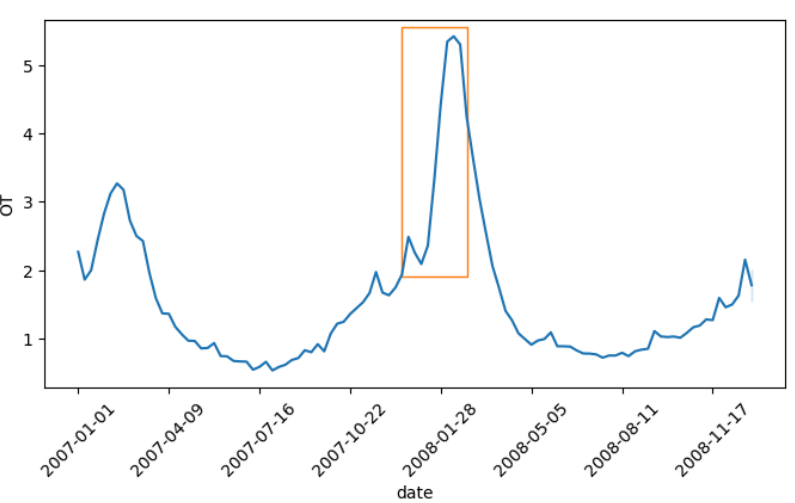
\includegraphics[width = \linewidth]{Figures/Neurips-CaseStudy.png}
    \caption{Case Study of Semantic Alignment from the Health Dataset.}
    \label{fig:alg}
\vspace{-3mm}
\end{figure}
\section{Details of \mmtsf}\label{app:lib}
In terms of implementation, \mmtsf chooses to extend the widely used Time-Series Library (TSlib)\footnote{https://github.com/thuml/Time-Series-Library}, thus ensuring ease of use. For LLM invocation, \mmtsf utilizes the popular and active Hugging Face\footnote{https://huggingface.co/models}. For the projection layer, we use a multilayer perceptron (MLP) to keep it simple, apply instance normalization followed by adjusting the mean to the corresponding historical average to keep it rational. We tune the initialization values of the linear weighting mechanism to prevent overfitting or reduce learning difficulty. To use \model dataset for TSF task, \mmtsf constrains the latest end date of the input text sequence to be earlier than the latest end date of the input sequence, in order to avoid information leakage. Overall, \mmtsf supports multimodal extensions of over 20 unimodal TSF algorithms via 7 open-source LLM models.

\subsection{List of Supported TSF}
So far, our models supports following TSF models: TimeMixer ~\cite{wang2024timemixer}, TSMixer ~\cite{chen2023tsmixer}, iTransformer ~\cite{liu2023itransformer}, PatchTST ~\cite{nie2022time}, TimesNet ~\cite{wu2023timesnet}, DLinear ~\cite{zeng2023transformers}, LightTS ~\cite{zhang2022less}, ETSformer ~\cite{woo2202etsformer}, Non-stationary Transformer ~\cite{liu2022non}, FEDformer ~\cite{zhou2022fedformer}, Pyraformer ~\cite{liu2021pyraformer}, Autoformer ~\cite{wu2021autoformer}, Informer ~\cite{zhou2021informer}, Reformer ~\cite{kitaev2020reformer}, Transformer ~\cite{vaswani2017attention}, Mamba ~\cite{gu2023mamba}, SegRNN ~\cite{lin2023segrnn}, Koopa ~\cite{liu2024koopa}, FreTS ~\cite{yi2024frequency}, TiDE ~\cite{das2023long}, FiLM ~\cite{zhou2022film}, MICN ~\cite{wang2022micn}, Crossformer ~\cite{zhang2022crossformer}, TFT ~\cite{lim2021temporal}.

\subsection{List of Supported LLM}
For LLM, \mmtsf supports BERT~\cite{devlin2018bert}, GPT-2~\cite{radford2019language} (Small, Medium, Large, Extra-Large), Llama-2-7B~\cite{touvron2023llama}, and Llama-3-8B\footnote{\url{https://llama.meta.com/llama3}}.

\section{More Details of Experimental Setup}\label{app:setup}
\subsection{Time-Series Forecasting Backbones}
%desciption with one centences; using my excel;
We deployed two sets of experiments upon TSF models: (1) Transformer-based, including Transformer ~\cite{vaswani2017attention}, Reformer ~\cite{kitaev2020reformer}, Informer ~\cite{zhou2021informer}, Autoformer ~\cite{wu2021autoformer}, Crossformer ~\cite{zhang2022crossformer}, Non-stationary Transformer ~\cite{liu2022non},FEDformer ~\cite{zhou2022fedformer}, iTransformer ~\cite{liu2023itransformer}. (2) MLP-based: DLinear ~\cite{zeng2023transformers}. (3) Agnostic: FiLM ~\cite{zhou2022film}. (4) LLM-based: Time-LLM~\cite{jin2023time}.

\begin{itemize}
    \item \textbf{Transformer}, a classic sequence-to-sequence model basing on multi-head attention mechanism.
    \item \textbf{Reformer}, an computational-efficient Transformer with advancements in attention hashing and reversible residual layers
    \item \textbf{Informer}, an advanced Transformer designed to tackle long-term forecasting problem with sparse attention layers and self-attention distilling.
    \item \textbf{Autoformer}, a Transformer-based model that keeps encoder-decoder structure but alters attention computations by auto-correlation mechanism in order to benefit long-term forecasting.
    \item \textbf{Crossformer}, a multi-variate Transformer-based model that explicitly explores and utilizes cross-dimension dependencies. 
    \item \textbf{Non-stationary Transformer}, a Transformer that is designed to capture non-stationarity patterns instead of temporal correlation.
    \item \textbf{FEDformer}, a Transformer that explicitly use Fourier decomposition results to enhance long-term forecasting ability.
    \item \textbf{iTransformer}, a inverted Transformer that tokenizes multivariate time-series upon each timestamps/
    \item \textbf{DLinear}, a linear model that performs forecasting by a direct regression upon historical time series with a one-layer linear model.
    \item \textbf{FiLM}, a model-agnostic method that introduces Legendre and Fourier projections to denoise series and approximate historical information.
    \item \textbf{Time-LLM}, a framework that integrates LLM for time-series forecasting by reprogramming input series and then aligning with text prototypes.
\end{itemize}

\subsection{LLM Backbones}

We use GPT-2 Small ~\cite{radford2019language} for the majority of experiments, while other GPT-2 models and BERT, Llama-2, and Llama-3 are used in the ablation study.

\begin{itemize}
    \item \textbf{BERT} a bidirectional transformer pre-trained on large text corpora with tasks like masked language modeling and next sentence prediction
    \item \textbf{GPT-2} an advanced language model that generates coherent and contextually relevant text by predicting subsequent words in a sentence, pre-trained on diverse internet text and capable of performing a variety of language tasks without task-specific fine-tuning
    \item \textbf{Llama-2} an accessible, open-source LLM designed to generate coherent and contextually relevant text by leveraging advanced transformer-based architecture 
    \item \textbf{Llama-3} the latest iteration of the Llama model, offering enhanced text generation and comprehension abilities, further advancing the performance and versatility of its predecessors
\end{itemize}

\subsection{Evaluation Metrics}\label{sec:metrics}
We use mean squared error (MSE) as the evaluation metric for all experiments. The MSE is defined as the average of the squares of the errors. The error here is the difference between the forecasted value $y_i$ and the actual value $\hat{y}_i$. That is:

\begin{equation}
\text{MSE} = \frac{1}{n} \sum_{i=1}^{n} (y_i - \hat{y}_i)^2
\end{equation}

\subsection{Details of Implementation}
We follow the commonly adopted setup for defining the forecasting horizon window length, as outlined in prior works~\cite{wu2021autoformer,wu2023timesnet,nie2022time}. Specifically, for daily reported datasets, the forecasting horizon windows are chosen from the set [48, 96, 192, 336], with a fixed lookback window size of 96 and a consistent label window size of 48 for the decoder. Similarly, for the weekly reported dataset, we employ forecasting horizon windows from [12, 24, 36, 48], with a fixed lookback window size of 36 and a constant label window size of 18 for the decoder. Besides, for the monthly reported dataset, we employ forecasting horizon windows from [6,8,10,12], with a fixed lookback window size of 8 and a constant label window size of 4 for the decoder. 

To avoid the time consumption of matching data one by one during training, we adopted a simple preprocessing method: tracing back the most recent k text samples based on the timestamp of the numerical sample to construct pre-stored pairs. We focused on the search text and retained the source, i.e., URL, to provide rich and formatted information. It is worth noting that this processing method is a simple preliminary exploration, and we look forward to more effective and efficient matching approaches tailored for time series forecasting tasks with our \model.
\section{Additional Experiments on Text Integration Approaches}\label{app:texti_inte}
The previously proposed multimodal integration approaches~\cite{jin2023time,cao2023tempo} are designed specifically for prompt-based text rather than exogenous textual series. Specifically, the text used in these models serves as prompts, such as task descriptions, rather than our exogenous textual series. Prompts are static, fixed in length, highly templated, and do not provide additional information, which makes them significantly different from the textual series used in our \model. We choose Time-LLM~\cite{jin2023time}, an advanced model in this category, as a representative. The experimental results are shown in Table~\ref{tab:MI}.
\begin{table}[h]
\centering
\begin{tabular}{cccc} 
\hline
\textbf{Model}          & \textbf{Health} & \textbf{Energy} & \textbf{Traffic}  \\ 
\hline
TimeLLM (Unimodal)            & 1.92            & 0.30            & 0.23              \\ 
TimeLLM (Multimodal\_TimeLLM) & 2.51            & 0.39            & 0.27              \\ 
TimeLLM (Multimodal\_Our)     & 1.42            & 0.25            & 0.22              \\
\hline
\end{tabular}
\caption{Results of Additional Experiments on Multimodal Integration Approaches\label{tab:MI}}

\end{table}


The results show that the 'prompt as prefix' approach in TimeLLM, referred to as Multimodal\_TimeLLM, is not suitable for handling textual series. Possible reasons include the longer length of the text series potentially overwhelming the numerical series information, among others. In contrast, our framework, although simple, proves to be effective."

We also empirically found that using only the embedding layer of the LLM to model text often achieves results close to or even better than the last layer. This is consistent with recent research findings~\cite{tan2024language}, validating that there is still significant room for improvement when using LLMs for time series forecasting.
\section{Additional Experiments on Text Modeling Approaches}\label{app:tm}
Results are provided in Table~\ref{tab:TI}.
\begin{table}
\centering
\begin{tabular}{cccc} 
\hline
Dataset                   & Health & Energy & Traffic  \\ 
\hline
Reformer (Uni)            & 1.85   & 0.43   & 0.31     \\ 
Reformer (Multi\_Bert)    & 1.27   & 0.40   & 0.17     \\ 
Reformer (Multi\_Doc2Vec) & 1.35   & 0.43   & 0.22     \\ 
Informer (Uni)            & 1.53   & 0.33   & 0.28     \\ 
Informer (Multi\_Bert)    & 1.22   & 0.29   & 0.17     \\ 
Informer (Multi\_Doc2Vec) & 1.32   & 0.31   & 0.21     \\
\hline
\end{tabular}
\caption{Results of Additional Text Modeling Solutions\label{tab:TI}}
\end{table}
\section{Additional Experiments on Multimodal Modeling Approaches}\label{app:mma}
\subsection{Using attention mechanisms}
We use the output of the time series model to calculate attention scores for each token in the LLM output and perform weighted aggregation. For detailed implementation, please refer to our library. Results are provided in Table~\ref{tab:AMM}. This basic attention method has not yet demonstrated a clear advantage over the current simple combing approach. We look forward to future method designs.
\begin{table}[h]
\centering
\begin{tabular}{cccc}
\hline
Dataset               & Health & Energy & Traffic \\ \hline
Reformer (Multi\_Our) & 1.27   & 0.41   & 0.17    \\
Reformer (Multi\_Att)  & 1.26   & 0.39   & 0.22    \\
Informer (Multi\_Our) & 1.22   & 0.29   & 0.17    \\
Informer (Multi\_Att)  & 1.23   & 0.29   & 0.16    \\ \hline
\end{tabular}
\caption{Results of Using Attention Mechanisms for Multimodal TSF\label{tab:AMM}}

\end{table}
\subsection{Using closed-source LLMs}
We first used closed-source LLMs, such as GPT-3.5, to generate text-based predictions, and then encoded them using BERT. For detailed implementation, please check our library. Results are provided in Table~\ref{tab:GPT}. We initially observed that fully frozen closed-source LLMs are less effective than fine-tuned open-source LLM.
\begin{table}[h]
\centering

\begin{tabular}{cccc}
\hline
Dataset                & Health & Energy & Traffic \\ \hline
Reformer (Uni)          & 1.86   & 0.43   & 0.31    \\
Reformer (Multi\_Bert)   & 1.27   & 0.40   & 0.17    \\
Reformer (Multi\_GPT3.5) & 1.38   & 0.46   & 0.19    \\
Informer (Uni)          & 1.53   & 0.33   & 0.28    \\
Informer (Multi\_Bert)   & 1.22   & 0.28   & 0.17    \\
Informer (Multi\_GPT3.5) & 1.33   & 0.32   & 0.23    \\ \hline
\end{tabular}
\caption{Results of Using Closed-Source LLMs for Multimodal TSF\label{tab:GPT}}

\end{table}

In addition, we empirically observe that using the encoder layers of LLMs usually yields better performance.
\newpage
\section{Detailed Results}\label{app:detailed_results}

\begin{table}[h]
\centering
\resizebox{\textwidth}{!}{
\begin{tabular}{cc|c|c|c|c}
\toprule
& Horizon Window Length& \multirow{2}{*}{6} & \multirow{2}{*}{8} & \multirow{2}{*}{10} & \multirow{2}{*}{12} \\ \cline{1-2}
Model & Modal & & & & \\
\midrule
\multirow{2}{*}{FiLM}& Uni & $0.07$ & $0.09$ & $0.12$ & $0.15$ \\
& Multi & $0.06$ & $0.09$ & $0.10$ & $0.14$ \\
\multirow{2}{*}{DLinear}& Uni & $0.11$ & $0.24$ & $0.18$ & $0.23$ \\
& Multi & $0.09$ & $0.17$ & $0.13$ & $0.16$ \\
\multirow{2}{*}{Transformer}& Uni & $0.24$ & $0.35$ & $0.40$ & $0.50$ \\
& Multi & $0.14$ & $0.16$ & $0.24$ & $0.24$ \\
\multirow{2}{*}{Reformer}& Uni & $0.38$ & $0.26$ & $0.51$ & $0.70$ \\
& Multi & $0.19$ & $0.18$ & $0.27$ & $0.32$ \\
\multirow{2}{*}{Informer}& Uni & $0.51$ & $0.61$ & $0.66$ & $0.80$ \\
& Multi & $0.16$ & $0.21$ & $0.34$ & $0.34$ \\
\multirow{2}{*}{Autoformer}& Uni & $0.08$ & $0.09$ & $0.11$ & $0.14$ \\
& Multi & $0.08$ & $0.09$ & $0.10$ & $0.13$ \\
\multirow{2}{*}{FEDformer}& Uni & $0.06$ & $0.08$ & $0.10$ & $0.13$ \\
& Multi & $0.06$ & $0.07$ & $0.10$ & $0.13$ \\
\multirow{2}{*}{\begin{tabular}[c]{c}Nonstationary\\Transformer\end{tabular}}& Uni & $0.06$ & $0.07$ & $0.10$ & $0.12$ \\
& Multi & $0.05$ & $0.07$ & $0.09$ & $0.12$ \\
\multirow{2}{*}{Crossformer}& Uni & $0.31$ & $0.35$ & $0.38$ & $0.46$ \\
& Multi & $0.11$ & $0.16$ & $0.20$ & $0.26$ \\
\multirow{2}{*}{PatchTST}& Uni & $0.06$ & $0.08$ & $0.10$ & $0.13$ \\
& Multi & $0.06$ & $0.08$ & $0.10$ & $0.13$ \\
\multirow{2}{*}{iTransformer}& Uni & $0.06$ & $0.08$ & $0.10$ & $0.13$ \\
& Multi & $0.06$ & $0.08$ & $0.10$ & $0.13$ \\
\multirow{2}{*}{Time-LLM}& Uni & $0.08$ & $0.09$ & $0.10$ & $0.14$ \\
& Multi & $0.06$ & $0.08$ & $0.10$ & $0.13$ \\
\bottomrule 
\end{tabular}}
\caption{Agriculture\label{tab:detailed_Agriculture}}
\end{table}

\begin{table}[h]
\centering
\resizebox{\textwidth}{!}{
\begin{tabular}{cc|c|c|c|c}
\toprule
& Horizon Window Length& \multirow{2}{*}{6} & \multirow{2}{*}{8} & \multirow{2}{*}{10} & \multirow{2}{*}{12} \\ \cline{1-2}
Model & Modal & & & & \\
\midrule
\multirow{2}{*}{FiLM}& Uni & $1.42$ & $1.39$ & $1.40$ & $1.40$ \\
& Multi & $1.15$ & $1.15$ & $1.14$ & $1.17$ \\
\multirow{2}{*}{DLinear}& Uni & $1.35$ & $1.41$ & $1.36$ & $1.36$ \\
& Multi & $1.06$ & $1.05$ & $1.07$ & $1.08$ \\
\multirow{2}{*}{Transformer}& Uni & $1.04$ & $1.14$ & $1.12$ & $1.11$ \\
& Multi & $0.97$ & $1.01$ & $1.00$ & $1.00$ \\
\multirow{2}{*}{Reformer}& Uni & $1.24$ & $1.06$ & $1.13$ & $1.16$ \\
& Multi & $0.97$ & $0.95$ & $0.94$ & $0.98$ \\
\multirow{2}{*}{Informer}& Uni & $1.08$ & $1.11$ & $1.08$ & $1.07$ \\
& Multi & $1.04$ & $1.03$ & $1.04$ & $1.02$ \\
\multirow{2}{*}{Autoformer}& Uni & $1.30$ & $1.24$ & $1.28$ & $1.25$ \\
& Multi & $1.08$ & $1.02$ & $1.05$ & $1.05$ \\
\multirow{2}{*}{FEDformer}& Uni & $1.32$ & $1.36$ & $1.28$ & $1.27$ \\
& Multi & $0.98$ & $1.00$ & $1.03$ & $1.02$ \\
\multirow{2}{*}{\begin{tabular}[c]{c}Nonstationary\\Transformer\end{tabular}}& Uni & $1.30$ & $1.32$ & $1.36$ & $1.32$ \\
& Multi & $1.00$ & $1.02$ & $1.02$ & $1.01$ \\
\multirow{2}{*}{Crossformer}& Uni & $1.12$ & $1.10$ & $1.12$ & $1.10$ \\
& Multi & $1.00$ & $0.99$ & $1.00$ & $1.01$ \\
\multirow{2}{*}{PatchTST}& Uni & $1.36$ & $1.33$ & $1.27$ & $1.28$ \\
& Multi & $0.99$ & $1.01$ & $1.04$ & $1.06$ \\
\multirow{2}{*}{iTransformer}& Uni & $1.16$ & $1.23$ & $1.24$ & $1.22$ \\
& Multi & $0.99$ & $1.01$ & $1.04$ & $1.06$ \\
\multirow{2}{*}{Time-LLM}& Uni & $1.36$ & $1.26$ & $1.27$ & $1.27$ \\
& Multi & $0.99$ & $1.01$ & $1.04$ & $1.07$ \\
\bottomrule 
\end{tabular}}
\caption{Climate\label{tab:detailed_Climate}}
\end{table}

\begin{table}[h]
\centering
\resizebox{\textwidth}{!}{
\begin{tabular}{cc|c|c|c|c}
\toprule
& Horizon Window Length& \multirow{2}{*}{6} & \multirow{2}{*}{8} & \multirow{2}{*}{10} & \multirow{2}{*}{12} \\ \cline{1-2}
Model & Modal & & & & \\
\midrule
\multirow{2}{*}{FiLM}& Uni & $0.04$ & $0.04$ & $0.03$ & $0.04$ \\
& Multi & $0.03$ & $0.03$ & $0.03$ & $0.03$ \\
\multirow{2}{*}{DLinear}& Uni & $0.08$ & $0.18$ & $0.10$ & $0.11$ \\
& Multi & $0.04$ & $0.10$ & $0.03$ & $0.03$ \\
\multirow{2}{*}{Transformer}& Uni & $0.60$ & $0.69$ & $1.19$ & $1.12$ \\
& Multi & $0.14$ & $0.31$ & $0.23$ & $0.36$ \\
\multirow{2}{*}{Reformer}& Uni & $0.65$ & $0.76$ & $1.02$ & $0.55$ \\
& Multi & $0.22$ & $0.21$ & $0.32$ & $0.28$ \\
\multirow{2}{*}{Informer}& Uni & $1.59$ & $1.82$ & $1.74$ & $2.08$ \\
& Multi & $0.28$ & $0.36$ & $0.49$ & $0.50$ \\
\multirow{2}{*}{Autoformer}& Uni & $0.08$ & $0.10$ & $0.07$ & $0.06$ \\
& Multi & $0.07$ & $0.08$ & $0.07$ & $0.07$ \\
\multirow{2}{*}{FEDformer}& Uni & $0.05$ & $0.06$ & $0.05$ & $0.06$ \\
& Multi & $0.04$ & $0.03$ & $0.04$ & $0.03$ \\
\multirow{2}{*}{\begin{tabular}[c]{c}Nonstationary\\Transformer\end{tabular}}& Uni & $0.02$ & $0.02$ & $0.02$ & $0.03$ \\
& Multi & $0.02$ & $0.02$ & $0.02$ & $0.02$ \\
\multirow{2}{*}{Crossformer}& Uni & $0.95$ & $1.06$ & $1.22$ & $1.24$ \\
& Multi & $0.17$ & $0.16$ & $0.27$ & $0.29$ \\
\multirow{2}{*}{PatchTST}& Uni & $0.02$ & $0.02$ & $0.02$ & $0.02$ \\
& Multi & $0.02$ & $0.02$ & $0.02$ & $0.02$ \\
\multirow{2}{*}{iTransformer}& Uni & $0.02$ & $0.02$ & $0.02$ & $0.02$ \\
& Multi & $0.01$ & $0.02$ & $0.02$ & $0.02$ \\
\multirow{2}{*}{Time-LLM}& Uni & $0.06$ & $0.08$ & $0.02$ & $0.05$ \\
& Multi & $0.02$ & $0.02$ & $0.02$ & $0.02$ \\
\bottomrule 
\end{tabular}}
\caption{Economy\label{tab:detailed_Economy}}
\end{table}

\begin{table}[h]
\centering
\resizebox{\textwidth}{!}{
\begin{tabular}{cc|c|c|c|c}
\toprule
& Horizon Window Length& \multirow{2}{*}{12} & \multirow{2}{*}{24} & \multirow{2}{*}{36} & \multirow{2}{*}{48} \\ \cline{1-2}
Model & Modal & & & & \\
\midrule
\multirow{2}{*}{FiLM}& Uni & $0.21$ & $0.30$ & $0.37$ & $0.49$ \\
& Multi & $0.17$ & $0.28$ & $0.36$ & $0.48$ \\
\multirow{2}{*}{DLinear}& Uni & $0.26$ & $0.32$ & $0.39$ & $0.50$ \\
& Multi & $0.22$ & $0.29$ & $0.36$ & $0.47$ \\
\multirow{2}{*}{Transformer}& Uni & $0.18$ & $0.26$ & $0.36$ & $0.44$ \\
& Multi & $0.13$ & $0.22$ & $0.32$ & $0.42$ \\
\multirow{2}{*}{Reformer}& Uni & $0.28$ & $0.38$ & $0.49$ & $0.57$ \\
& Multi & $0.25$ & $0.38$ & $0.43$ & $0.54$ \\
\multirow{2}{*}{Informer}& Uni & $0.18$ & $0.29$ & $0.35$ & $0.48$ \\
& Multi & $0.15$ & $0.24$ & $0.32$ & $0.44$ \\
\multirow{2}{*}{Autoformer}& Uni & $0.18$ & $0.31$ & $0.34$ & $0.47$ \\
& Multi & $0.16$ & $0.27$ & $0.32$ & $0.45$ \\
\multirow{2}{*}{FEDformer}& Uni & $0.11$ & $0.24$ & $0.34$ & $0.45$ \\
& Multi & $0.09$ & $0.21$ & $0.32$ & $0.44$ \\
\multirow{2}{*}{\begin{tabular}[c]{c}Nonstationary\\Transformer\end{tabular}}& Uni & $0.11$ & $0.21$ & $0.34$ & $0.48$ \\
& Multi & $0.10$ & $0.20$ & $0.28$ & $0.46$ \\
\multirow{2}{*}{Crossformer}& Uni & $0.14$ & $0.29$ & $0.36$ & $0.41$ \\
& Multi & $0.13$ & $0.26$ & $0.36$ & $0.41$ \\
\multirow{2}{*}{PatchTST}& Uni & $0.10$ & $0.21$ & $0.30$ & $0.42$ \\
& Multi & $0.10$ & $0.21$ & $0.29$ & $0.41$ \\
\multirow{2}{*}{iTransformer}& Uni & $0.10$ & $0.21$ & $0.30$ & $0.42$ \\
& Multi & $0.09$ & $0.19$ & $0.29$ & $0.41$ \\
\multirow{2}{*}{Time-LLM}& Uni & $0.16$ & $0.27$ & $0.31$ & $0.45$ \\
& Multi & $0.10$ & $0.20$ & $0.29$ & $0.41$ \\
\bottomrule 
\end{tabular}}
\caption{Energy\label{tab:detailed_Energy}}
\end{table}

\begin{table}[h]
\centering
\resizebox{\textwidth}{!}{
\begin{tabular}{cc|c|c|c|c}
\toprule
& Horizon Window Length& \multirow{2}{*}{48} & \multirow{2}{*}{96} & \multirow{2}{*}{192} & \multirow{2}{*}{336} \\ \cline{1-2}
Model & Modal & & & & \\
\midrule
\multirow{2}{*}{FiLM}& Uni & $0.32$ & $0.35$ & $0.35$ & $0.32$ \\
& Multi & $0.30$ & $0.32$ & $0.32$ & $0.30$ \\
\multirow{2}{*}{DLinear}& Uni & $0.41$ & $0.57$ & $0.73$ & $0.59$ \\
& Multi & $0.32$ & $0.40$ & $0.46$ & $0.42$ \\
\multirow{2}{*}{Transformer}& Uni & $0.32$ & $0.32$ & $0.48$ & $0.44$ \\
& Multi & $0.59$ & $0.61$ & $0.70$ & $0.32$ \\
\multirow{2}{*}{Reformer}& Uni & $0.39$ & $0.45$ & $0.51$ & $0.48$ \\
& Multi & $0.29$ & $0.35$ & $0.36$ & $0.32$ \\
\multirow{2}{*}{Informer}& Uni & $0.39$ & $0.42$ & $0.46$ & $0.48$ \\
& Multi & $0.31$ & $0.33$ & $0.39$ & $0.34$ \\
\multirow{2}{*}{Autoformer}& Uni & $0.43$ & $0.36$ & $0.52$ & $0.37$ \\
& Multi & $0.35$ & $0.35$ & $0.35$ & $0.34$ \\
\multirow{2}{*}{FEDformer}& Uni & $0.36$ & $0.43$ & $0.42$ & $0.35$ \\
& Multi & $0.30$ & $0.34$ & $0.34$ & $0.33$ \\
\multirow{2}{*}{\begin{tabular}[c]{c}Nonstationary\\Transformer\end{tabular}}& Uni & $0.31$ & $0.39$ & $0.43$ & $0.38$ \\
& Multi & $0.29$ & $0.31$ & $0.32$ & $0.30$ \\
\multirow{2}{*}{Crossformer}& Uni & $0.34$ & $0.33$ & $0.73$ & $0.53$ \\
& Multi & $0.29$ & $0.30$ & $0.36$ & $0.36$ \\
\multirow{2}{*}{PatchTST}& Uni & $0.35$ & $0.38$ & $0.36$ & $0.32$ \\
& Multi & $0.31$ & $0.32$ & $0.32$ & $0.30$ \\
\multirow{2}{*}{iTransformer}& Uni & $0.28$ & $0.29$ & $0.30$ & $0.28$ \\
& Multi & $0.28$ & $0.29$ & $0.29$ & $0.27$ \\
\multirow{2}{*}{Time-LLM}& Uni & $0.38$ & $0.37$ & $0.45$ & $0.33$ \\
& Multi & $0.29$ & $0.30$ & $0.31$ & $0.28$ \\
\bottomrule 
\end{tabular}}
\caption{Environment\label{tab:detailed_Environment}}
\end{table}

\begin{table}[h]
\centering
\resizebox{\textwidth}{!}{
\begin{tabular}{cc|c|c|c|c}
\toprule
& Horizon Window Length& \multirow{2}{*}{12} & \multirow{2}{*}{24} & \multirow{2}{*}{36} & \multirow{2}{*}{48} \\ \cline{1-2}
Model & Modal & & & & \\
\midrule
\multirow{2}{*}{FiLM}& Uni & $2.53$ & $2.59$ & $2.46$ & $2.38$ \\
& Multi & $1.67$ & $1.83$ & $1.80$ & $1.81$ \\
\multirow{2}{*}{DLinear}& Uni & $2.37$ & $2.61$ & $2.50$ & $2.48$ \\
& Multi & $1.62$ & $1.67$ & $1.68$ & $1.78$ \\
\multirow{2}{*}{Transformer}& Uni & $1.22$ & $1.56$ & $1.43$ & $1.55$ \\
& Multi & $0.93$ & $1.34$ & $1.26$ & $1.29$ \\
\multirow{2}{*}{Reformer}& Uni & $1.63$ & $1.99$ & $1.91$ & $1.90$ \\
& Multi & $1.06$ & $1.30$ & $1.33$ & $1.39$ \\
\multirow{2}{*}{Informer}& Uni & $1.24$ & $1.61$ & $1.61$ & $1.67$ \\
& Multi & $0.98$ & $1.23$ & $1.28$ & $1.40$ \\
\multirow{2}{*}{Autoformer}& Uni & $1.99$ & $2.25$ & $2.26$ & $2.39$ \\
& Multi & $1.43$ & $1.74$ & $1.76$ & $1.69$ \\
\multirow{2}{*}{FEDformer}& Uni & $1.08$ & $1.58$ & $1.69$ & $1.76$ \\
& Multi & $0.92$ & $1.25$ & $1.36$ & $1.42$ \\
\multirow{2}{*}{\begin{tabular}[c]{c}Nonstationary\\Transformer\end{tabular}}& Uni & $1.19$ & $1.68$ & $1.91$ & $2.02$ \\
& Multi & $0.94$ & $1.14$ & $1.17$ & $1.30$ \\
\multirow{2}{*}{Crossformer}& Uni & $1.45$ & $1.57$ & $1.62$ & $1.65$ \\
& Multi & $1.01$ & $1.29$ & $1.28$ & $1.37$ \\
\multirow{2}{*}{PatchTST}& Uni & $1.23$ & $1.63$ & $1.78$ & $1.86$ \\
& Multi & $0.98$ & $1.27$ & $1.49$ & $1.60$ \\
\multirow{2}{*}{iTransformer}& Uni & $1.14$ & $1.62$ & $1.84$ & $1.89$ \\
& Multi & $0.97$ & $1.38$ & $1.71$ & $1.72$ \\
\multirow{2}{*}{Time-LLM}& Uni & $1.60$ & $1.94$ & $1.95$ & $2.17$ \\
& Multi & $0.98$ & $1.36$ & $1.65$ & $1.69$ \\
\bottomrule 
\end{tabular}}
\caption{Health(US)\label{tab:detailed_Health}}
\end{table}

\begin{table}[h]
\centering
\resizebox{\textwidth}{!}{
\begin{tabular}{cc|c|c|c|c}
\toprule
& Horizon Window Length& \multirow{2}{*}{6} & \multirow{2}{*}{8} & \multirow{2}{*}{10} & \multirow{2}{*}{12} \\ \cline{1-2}
Model & Modal & & & & \\
\midrule
\multirow{2}{*}{FiLM}& Uni & $127.92$ & $122.53$ & $125.10$ & $127.06$ \\
& Multi & $105.92$ & $107.25$ & $109.80$ & $110.94$ \\
\multirow{2}{*}{DLinear}& Uni & $107.12$ & $111.72$ & $114.42$ & $116.65$ \\
& Multi & $104.28$ & $106.76$ & $108.53$ & $109.90$ \\
\multirow{2}{*}{Transformer}& Uni & $128.42$ & $130.78$ & $131.65$ & $133.04$ \\
& Multi & $122.54$ & $126.66$ & $125.95$ & $127.46$ \\
\multirow{2}{*}{Reformer}& Uni & $124.48$ & $125.68$ & $126.51$ & $127.26$ \\
& Multi & $122.11$ & $123.85$ & $124.54$ & $125.01$ \\
\multirow{2}{*}{Informer}& Uni & $129.43$ & $131.43$ & $132.84$ & $133.54$ \\
& Multi & $121.81$ & $124.24$ & $126.98$ & $126.73$ \\
\multirow{2}{*}{Autoformer}& Uni & $125.67$ & $119.82$ & $119.72$ & $126.67$ \\
& Multi & $107.95$ & $114.98$ & $113.34$ & $116.33$ \\
\multirow{2}{*}{FEDformer}& Uni & $114.98$ & $112.14$ & $117.92$ & $121.90$ \\
& Multi & $109.28$ & $109.55$ & $115.99$ & $117.22$ \\
\multirow{2}{*}{\begin{tabular}[c]{c}Nonstationary\\Transformer\end{tabular}}& Uni & $105.77$ & $106.90$ & $109.72$ & $111.16$ \\
& Multi & $104.15$ & $105.99$ & $110.49$ & $110.69$ \\
\multirow{2}{*}{Crossformer}& Uni & $124.70$ & $124.97$ & $127.49$ & $128.47$ \\
& Multi & $120.99$ & $122.40$ & $124.34$ & $125.50$ \\
\multirow{2}{*}{PatchTST}& Uni & $107.31$ & $111.42$ & $114.90$ & $113.11$ \\
& Multi & $108.75$ & $111.26$ & $114.61$ & $114.67$ \\
\multirow{2}{*}{iTransformer}& Uni & $113.20$ & $115.26$ & $116.32$ & $117.59$ \\
& Multi & $114.58$ & $116.49$ & $116.25$ & $116.31$ \\
\multirow{2}{*}{Time-LLM}& Uni & $112.96$ & $116.53$ & $116.46$ & $119.60$ \\
& Multi & $110.86$ & $114.54$ & $115.56$ & $115.63$ \\
\bottomrule 
\end{tabular}}
\caption{Security\label{tab:detailed_Security}}
\end{table}

\begin{table}[h]
\centering
\resizebox{\textwidth}{!}{
\begin{tabular}{cc|c|c|c|c}
\toprule
& Horizon Window Length& \multirow{2}{*}{6} & \multirow{2}{*}{8} & \multirow{2}{*}{10} & \multirow{2}{*}{12} \\ \cline{1-2}
Model & Modal & & & & \\
\midrule
\multirow{2}{*}{FiLM}& Uni & $1.03$ & $1.07$ & $1.16$ & $1.24$ \\
& Multi & $0.87$ & $0.97$ & $1.05$ & $1.06$ \\
\multirow{2}{*}{DLinear}& Uni & $1.01$ & $1.13$ & $1.20$ & $1.24$ \\
& Multi & $0.91$ & $1.02$ & $1.14$ & $1.15$ \\
\multirow{2}{*}{Transformer}& Uni & $0.78$ & $0.93$ & $0.98$ & $1.02$ \\
& Multi & $0.73$ & $0.84$ & $0.91$ & $0.90$ \\
\multirow{2}{*}{Reformer}& Uni & $0.81$ & $0.90$ & $0.96$ & $1.05$ \\
& Multi & $0.80$ & $0.85$ & $0.95$ & $1.03$ \\
\multirow{2}{*}{Informer}& Uni & $0.77$ & $0.86$ & $0.93$ & $0.94$ \\
& Multi & $0.74$ & $0.79$ & $0.86$ & $0.85$ \\
\multirow{2}{*}{Autoformer}& Uni & $0.89$ & $1.05$ & $1.05$ & $1.17$ \\
& Multi & $0.88$ & $0.96$ & $1.04$ & $1.12$ \\
\multirow{2}{*}{FEDformer}& Uni & $0.81$ & $0.92$ & $1.02$ & $1.11$ \\
& Multi & $0.80$ & $0.91$ & $0.98$ & $1.04$ \\
\multirow{2}{*}{\begin{tabular}[c]{c}Nonstationary\\Transformer\end{tabular}}& Uni & $0.85$ & $1.17$ & $1.29$ & $1.31$ \\
& Multi & $0.78$ & $1.08$ & $1.16$ & $1.23$ \\
\multirow{2}{*}{Crossformer}& Uni & $0.79$ & $0.83$ & $0.97$ & $0.94$ \\
& Multi & $0.75$ & $0.83$ & $0.89$ & $0.93$ \\
\multirow{2}{*}{PatchTST}& Uni & $0.88$ & $0.99$ & $1.07$ & $1.18$ \\
& Multi & $0.82$ & $0.92$ & $1.02$ & $1.10$ \\
\multirow{2}{*}{iTransformer}& Uni & $1.03$ & $1.11$ & $1.21$ & $1.22$ \\
& Multi & $0.90$ & $1.08$ & $1.12$ & $1.15$ \\
\multirow{2}{*}{Time-LLM}& Uni & $0.90$ & $1.00$ & $1.07$ & $1.19$ \\
& Multi & $0.90$ & $0.99$ & $1.08$ & $1.10$ \\
\bottomrule 
\end{tabular}}
\caption{SocialGood\label{tab:detailed_SocialGood}}
\end{table}

\begin{table}[h]
\centering
\resizebox{\textwidth}{!}{
\begin{tabular}{cc|c|c|c|c}
\toprule
& Horizon Window Length& \multirow{2}{*}{6} & \multirow{2}{*}{8} & \multirow{2}{*}{10} & \multirow{2}{*}{12} \\ \cline{1-2}
Model & Modal & & & & \\
\midrule
\multirow{2}{*}{FiLM}& Uni & $0.28$ & $0.28$ & $0.27$ & $0.31$ \\
& Multi & $0.25$ & $0.24$ & $0.24$ & $0.29$ \\
\multirow{2}{*}{DLinear}& Uni & $0.35$ & $0.42$ & $0.34$ & $0.38$ \\
& Multi & $0.28$ & $0.30$ & $0.25$ & $0.31$ \\
\multirow{2}{*}{Transformer}& Uni & $0.29$ & $0.29$ & $0.29$ & $0.29$ \\
& Multi & $0.15$ & $0.15$ & $0.16$ & $0.18$ \\
\multirow{2}{*}{Reformer}& Uni & $0.31$ & $0.28$ & $0.31$ & $0.33$ \\
& Multi & $0.16$ & $0.16$ & $0.17$ & $0.19$ \\
\multirow{2}{*}{Informer}& Uni & $0.26$ & $0.27$ & $0.27$ & $0.30$ \\
& Multi & $0.15$ & $0.16$ & $0.17$ & $0.18$ \\
\multirow{2}{*}{Autoformer}& Uni & $0.20$ & $0.20$ & $0.20$ & $0.29$ \\
& Multi & $0.19$ & $0.19$ & $0.20$ & $0.27$ \\
\multirow{2}{*}{FEDformer}& Uni & $0.21$ & $0.21$ & $0.20$ & $0.27$ \\
& Multi & $0.16$ & $0.16$ & $0.17$ & $0.23$ \\
\multirow{2}{*}{\begin{tabular}[c]{c}Nonstationary\\Transformer\end{tabular}}& Uni & $0.19$ & $0.21$ & $0.20$ & $0.27$ \\
& Multi & $0.19$ & $0.20$ & $0.19$ & $0.25$ \\
\multirow{2}{*}{Crossformer}& Uni & $0.25$ & $0.24$ & $0.25$ & $0.26$ \\
& Multi & $0.17$ & $0.16$ & $0.17$ & $0.19$ \\
\multirow{2}{*}{PatchTST}& Uni & $0.21$ & $0.21$ & $0.22$ & $0.28$ \\
& Multi & $0.18$ & $0.19$ & $0.20$ & $0.27$ \\
\multirow{2}{*}{iTransformer}& Uni & $0.20$ & $0.21$ & $0.22$ & $0.28$ \\
& Multi & $0.19$ & $0.20$ & $0.21$ & $0.27$ \\
\multirow{2}{*}{Time-LLM}& Uni & $0.21$ & $0.21$ & $0.21$ & $0.27$ \\
& Multi & $0.19$ & $0.20$ & $0.20$ & $0.27$ \\
\bottomrule 
\end{tabular}}
\caption{Traffic\label{tab:detailed_Traffic}}
\end{table}
\clearpage
\newpage
%jsut dataset; as mentioned new dataset need XXXXX
\section{Dataset Documentations}

The dataset is provided in \texttt{csv} format.

Each numerical data point contains the following attribute: 
\begin{itemize}
    \item start time
    \item end time
    \item values of target variables
    \item values of other variables
\end{itemize}
Each textual data point contains the following attribute: 
\begin{itemize}
    \item start time
    \item end time
    \item extracted fact text (content \& data source)
    \item extracted prediction text (content \& data source)
\end{itemize}

\section{Intended Uses}

\model is intended for researchers in machine learning and related fields to develop novel methods for multimodal time-series analysis. We also aim to help developers to train or fine-tune multi-modal foundation time-series models using our dataset.

\section{Accessing}

\model is publicly available in \url{https://github.com/AdityaLab/Time-MMD}. 
 A detailed demo on how the dataset can be read and used can be found at \url{https://github.com/AdityaLab/MM-TSFlib}. A Croissant card of \model can be found in \href{https://drive.google.com/file/d/1XGnCv6UVTGujWr6CwGFpg9_-qxPeniOb/view?usp=sharing}{Google Drive}.
\section{Statement}

The authors will bear all responsibility in case of violation of rights.

\section{Hosting and Maintenance Plan}

\model is hosted and version-tracked via GitHub. It will be permanently available under the link \url{https://github.com/AdityaLab/Time-MMD}. The download link of all the datasets can be found in the GitHub repository. We plan to regularly update the cutoff time of the data in \model at a frequency of every 6 months.

\section{\model Community}

\model is a community-driven and open-source initiative. We are committed and have resources to maintain and actively develop \model in the future. We plan to grow \model to include more languages, domains, and multimodal time series analysis tasks. We welcome external contributors.


\section{Licensing}

We license our dataset by \href{http://opendatacommons.org/licenses/by/1.0/}{ODC-By v1.0}. While parsing the data, we follow the terms of both Google Search API\footnote{\url{https://developers.google.com/terms}} and WebScraper\footnote{\url{https://webscraper.io/extension-privacy-policy}}. We further make sure that all data sources obtained in \model are in public domain and authorized for non-commercial distribution. The authors will bear all responsibility in case of violation of rights.